\documentclass[referee,useAMS,usenatbib]{biom}

\usepackage{amsmath}
\usepackage{amssymb}
\usepackage{graphicx}
\usepackage{floatpag}
\usepackage{bm}
\usepackage[nameinlink,capitalise,noabbrev]{cleveref}
\usepackage{csquotes}
\usepackage[T1]{fontenc}
\usepackage{textcomp} % provide symbols
\usepackage{xr}
\usepackage{afterpage}
\usepackage{caption}
\usepackage{numprint}
\usepackage{url}
\npfourdigitnosep
\npdecimalsign{.}

% Generic maths commands
\def\reals{\mathbb{R}}
\def\nats{\mathbb{N}}
\def\sampSpace{\mathcal{X}}
\def\dist{\sim}
\DeclareMathOperator{\E}{\mathbb{E}}
\DeclareMathOperator{\V}{\mathbb{V}}
\DeclareMathOperator{\I}{\mathbb{I}}
\newcommand{\ind}{\mathrel{\perp\!\!\!\perp}}
\DeclareMathOperator{\prob}{\mathrm{Pr}}
\DeclareMathOperator{\p}{\pi}
\DeclareMathOperator{\var}{\mathbb{V}}
\DeclareMathOperator{\indicator}{\mathbb{I}}
\DeclareMathOperator{\cov}{Cov}
\DeclareMathOperator{\cor}{Cor}
\DeclareMathOperator{\logit}{logit}
\DeclareMathOperator{\Ber}{Bernoulli}
\DeclareMathOperator{\Bin}{Binomial}
\DeclareMathOperator{\Poi}{Poisson}
\DeclareMathOperator{\BetaDist}{Beta}
\DeclareMathOperator{\Exponential}{Exponential}
\DeclareMathOperator{\NBr}{NegBin}
\newcommand{\NBc}{\NBr}
\DeclareMathOperator{\BB}{BetaBin}
\DeclareMathOperator{\GamDist}{Gamma}
\DeclareMathOperator{\MN}{Multinomial}
\DeclareMathOperator{\N}{N}
\DeclareMathOperator{\MNorm}{N}
\DeclareMathOperator{\LN}{LN}
\DeclareMathOperator{\LKJ}{LKJ}
\DeclareMathOperator{\expit}{expit}
\newcommand\matr{\bm}
\newcommand\set{\mathcal}
\renewcommand{\vec}[1]{\bm{#1}}
\newcommand{\ssep}{:}
\DeclareMathOperator*{\argmax}{arg\,max}

\newcommand\citePersonalComms[1]{(#1, personal communication)}

% Thesis-specific maths commands
\newcommand{\dmax}{d_\text{max}}
\newcommand{\psens}{p_\text{sens}}
\newcommand{\psenss}{p_\text{sens}^{(s)}}
\newcommand{\psensi}{p_\text{sens}^{(i)}}
\newcommand{\ntot}{n_\text{tot}}
\newcommand{\ndet}{n_\text{d}}
\newcommand{\nnodet}{n_\text{u}}
\newcommand{\pnodet}{p_\text{u}}
\newcommand{\Npop}{N_\text{pop}}
\newcommand{\Ncis}{N_\text{CIS}}
\newcommand{\ncis}{\vec{n_\text{CIS}}}
\newcommand{\na}{\vec{n}_\text{obs}}
\newcommand{\pcis}{\vec{p_\text{CIS}}}
\newcommand{\sched}{\mathcal{T}}
\newcommand{\nsched}{|\sched{}|}
\newcommand{\inform}{{_{\text{inform}}}}
\newcommand{\posResults}{r_{+}}
\newcommand{\negResults}{r_{-}}


% Macros for common abbreviations to get the spacing right
% See: https://stackoverflow.com/questions/3282319/correct-way-to-define-macros-etc-ie-in-latex
\usepackage{xspace}
\makeatletter
\DeclareRobustCommand\onedot{\futurelet\@let@token\@onedot}
\def\@onedot{\ifx\@let@token.\else.\null\fi\xspace}
\def\eg{e.g\onedot} \def\Eg{{E.g}\onedot}
\def\ie{i.e\onedot} \def\Ie{{I.e}\onedot}
\def\cf{c.f\onedot} \def\Cf{{C.f}\onedot}
\def\etc{etc\onedot} \def\vs{{vs}\onedot}
\def\wrt{w.r.t\onedot} \def\dof{d.o.f\onedot}
\def\etal{et al\onedot}
\makeatother

%----Helper code for dealing with external references----
% (by cyberSingularity at http://tex.stackexchange.com/a/69832/226)

\usepackage{xr}
\makeatletter

\newcommand*{\addFileDependency}[1]{% argument=file name and extension
\typeout{(#1)}% latexmk will find this if $recorder=0
% however, in that case, it will ignore #1 if it is a .aux or 
% .pdf file etc and it exists! If it doesn't exist, it will appear 
% in the list of dependents regardless)
%
% Write the following if you want it to appear in \listfiles 
% --- although not really necessary and latexmk doesn't use this
%
\@addtofilelist{#1}
%
% latexmk will find this message if #1 doesn't exist (yet)
\IfFileExists{#1}{}{\typeout{No file #1.}}
}\makeatother

\newcommand*{\myexternaldocument}[1]{%
\externaldocument{#1}%
\addFileDependency{#1.aux}%
\addFileDependency{#1.tex}%
}
\myexternaldocument{main}
%------------End of helper code--------------


\begin{document}

%\bibliographystyle{natbib}

\def\spacingset#1{\renewcommand{\baselinestretch}%
{#1}\small\normalsize} \spacingset{1}


%%%%%%%%%%%%%%%%%%%%%%%%%%%%%%%%%%%%%%%%%%%%%%%%%%%%%%%%%%%%%%%%%%%%%%%%%%%%%%


\appendix

\section{Derivations of quantities in \cref{sec:inference}} \label{sec:derivations}

\subsection{Derivation of posterior density} \label{sec:full-posterior-density}
As we assume independence:
\begin{align}
  \vec{n} \mid \ntot, \vec{\theta} &\dist \MN(\ntot, \vec{p})
\intertext{that is:}
  p(\vec{n} \mid \ntot, \vec{\theta}) &= \frac{\ntot!}{\nnodet!\prod_{k=1}^{N_E} n_k!} p_u^{\nnodet} \prod_{k=1}^{N_E} p_k^{n_k}.
  \label{perf-test:eq:multinomial-ll}
\end{align}

In the CIS data, each $n_k$ ($k \neq u$) is observed as either 0 or 1.
Define $\set{D} = \{ k \ssep n_k = 1 \}$, the set of detected episodes.
Furthermore, note that the support of the multinomial distribution requires that $\nnodet = \ntot - \ndet$.
Then \cref{perf-test:eq:multinomial-ll} simplifies to:
\begin{align}
  p(\vec{n} \mid \ntot, \vec{\theta})
  &= p(\na \mid \ntot, \vec{\theta}) \\
  &= \frac{\ntot!}{(\ntot - \ndet)!} p_u^{\ntot-\ndet} \prod_{k \in \set{D}} p_k.
  \label{perf-test:eq:multinomial}
\end{align}

The relevant information from the CIS data is fully contained in the vector $\na$.
Therefore, the posterior of interest is (full derivations of this and subsequent quantities are in \cref{sec:derivations}):
\begin{align}
p(\vec{\theta} \mid \na)
&\propto  p(\vec{\theta}) \left( \prod_{k \in \set{D}} p_k \right) \left( \sum_{\ntot=\ndet}^\infty p(\ntot \mid \vec{\theta}) \frac{\ntot!}{(\ntot - \ndet)!} \pnodet^{\ntot - \ndet} \right).
\label{perf-test:eq:posterior1}
\end{align}

For mathematical convenience, we assume the prior $\ntot \dist \NBc(\mu, r)$ (where $\mu$ is the prior mean and $r$ its overdispersion), and that it is independent of $\vec{\theta}$, the parameters of the survival distribution.
In this case \cref{perf-test:eq:posterior1} simplifies to:
\begin{align}
p(\vec{\theta} \mid \na)
&\propto p(\vec{\theta}) \left( \prod_{i \in \set{D}} p_k \right) (r + \mu (1- \pnodet))^{-(r+\ndet)} \label{perf-test:eq:full-posterior}.
\end{align}

\subsection{Deriving $1 - p_u$} \label{sec:derive-prob-undetected}

The final component of \cref{perf-test:eq:full-posterior} required is $1 - p_u$.
\Cref{sec:derivations} shows that
\begin{align}
  1 - p_u
  &= \frac{1}{\Ncis} \sum_{i=1}^{\Ncis} (1 - \prob(O_j = \varnothing \mid i_j = i, \vec{\theta})).
  \label{perf-test:eq:pu}
\end{align}
%% assuming $P(i_j = i \mid \vec{\theta}) = 1/\Ncis$ as before.
Let $p_{iu} = \prob(O_j = \varnothing \mid i_j = i, \vec{\theta})$.
%% Therefore, the crucial component is $1 - p_{iu}$.
%% This is one minus the probability that an episode in individual $i$ was undetected, \ie the probability of the episode being detected.
An episode $j$ in individual $i_j$ is detected if and only if all the following conditions are met.
\begin{enumerate}
    \item 
    $t\in[B_j, E_j]$ for some $t \in \sched_{i_j}$;
    % $\exists t \in \sched_{i_j}$ such that $b_j \leq t \leq e_j$; 
    \ie there is at least one positive test for the episode.
    \item $B_j > \min ( \sched_{i_j} )$.
      For individuals enrolled during the period considered ($\min \sched_{i_j} > 0$), this ensures that the beginning of the episode is lower bounded.
      For individuals enrolled prior to the period considered ($\min \sched_{i_j} \leq 0$), this means that the episode was not detected prior to time 1.
    \item $B_j \leq T_{i_j}$ where $T_{i_j} = \max \{ t \in \sched_{i_j} \ssep t \leq T \}$ is the last time that $i_j$ is tested in the period, meaning that the test is detected within the period.
    \item $\exists t \in \sched_{i_j}$ such that $t > E_j$, upper bounding the end of the episode.
      For episodes detected in the period we consider, a negligible number of episodes are excluded due to this criteria (<5\% of detected episodes, themselves likely around 15\% of all episodes).
      Therefore, we assume this occurs with probability 0.
      % For a new context, including recent infections, this condition could be relaxed by considering episodes that do not meet this criterion as right censored.
\end{enumerate}

% An episode is undetected if and only if no tests are performed during the episode or if there was no negative test prior to the episode.
% Equivalently, that the first test at or after $b$ is after $e$, or that there is no negative test prior to $b$.
First define $\tau_{\sched_i}(t)$ as the time until the next test at or after time $t$ in the schedule $\sched_i$:
\begin{align}
\tau_{\sched_i}(t) &= \min \{ t' \in \sched_i : t' \geq t \} - t
\label{perf-test:eq:tau-def}
\end{align}
% defining $\min \varnothing = \infty$; \ie $\tau_{\sched_i}(t) = \infty$ if there is no $t' \in \sched_i$ such that $t' \geq t$.
The first condition can now be expressed as $e_j \geq b_j + \tau_{\sched_{i_j}}(b_j)$.
Equivalently, $d_j \geq \tau_{\sched_{i_j}}(b_j) + 1$.
% The fourth condition can be expressed as $\tau_{\sched_{i_j}}(b_j) < \infty$.
% Then $\Omega_i$ can be written as:
% \begin{align}
% \Omega_i = \{ (b, e) \ssep \tau_{\sched_i}(b) + b > e \vee b \leq \min(\sched_i) \}.
% \end{align}
Therefore, omitting the conditioning on $\vec{\theta}$ and $i_j = i$:
\begin{align}
1 - p_{iu}
% &= 1 - \prob((B_{j}, E_{j}) \in \Omega_i) \\
&= \prob(D_j \geq \tau_{\sched_{i}}(B_j)+ 1, \min \sched_{i} < B_j \leq T_{i}) \\
&= \sum_{b = \min \sched_{i} + 1}^{T_{i}} \prob(D_j \geq \tau_{\sched_{i}}(b) + 1 \mid B_j = b) \prob(B_j = b)\\
&\propto \sum_{b = \min \sched_{i} + 1}^{T_{i}} S_{\vec{\theta}}(\tau_{\sched_{i}}(b) + 1).
\label{perf-test:eq:piu}
\end{align}


\subsection{Expressions in \cref{sec:inference}}

First, the derivation of $p(\vec{\theta} \mid \na)$:
\begin{align}
p(\vec{\theta} \mid \na)
&\propto p(\vec{\theta}) p(\na \mid \vec{\theta}) \\
&= p(\vec\theta) \sum_{\ntot= \ndet}^{\infty} p(\ntot, \na \mid \vec{\theta}) \\
&= p(\vec{\theta}) \sum_{\ntot=\ndet}^\infty p(\ntot \mid \vec{\theta}) p(\na \mid \ntot, \vec{\theta}) \\
&= p(\vec{\theta}) \sum_{\ntot=\ndet}^\infty p(\ntot \mid \vec{\theta}) \frac{\ntot!}{(\ntot - \ndet)!} \pnodet^{\ntot - \ndet} \prod_{k \in \set{D}} p_k &\text{by \cref{perf-test:eq:multinomial}} \\
&= p(\vec{\theta}) \left( \prod_{k \in \set{D}} p_k \right) \left( \sum_{\ntot=\ndet}^\infty p(\ntot \mid \vec{\theta}) \frac{\ntot!}{(\ntot - \ndet)!} \pnodet^{\ntot - \ndet} \right).
\intertext{For convenience, define the summation term as:}
\eta &= 
\sum_{\ntot=\ndet}^\infty p(\ntot \mid \vec{\theta}) \frac{\ntot!}{(\ntot - \ndet)!} \pnodet^{\ntot - \ndet}. \label{perf-test:eq:eta}
\end{align}

Next, we derive an analytical solution to $\eta$ (defined in \cref{perf-test:eq:eta}) assuming the prior $\ntot \dist \NBc(\mu, r)$, and that it is independent of $\vec{\theta}$, the parameters of the survival distribution.
Therefore, $p(\ntot \mid \vec{\theta}) = p(\ntot)$.
This assumption makes $\eta$ analytically tractable, allowing computationally feasible inference.

Putting a negative binomial prior on $\ntot$ is equivalent to the following gamma-Poisson composite; its use simplifies the derivation.
\begin{align}
\ntot \mid \lambda &\dist \Poi(\lambda) \\
\lambda &\dist \GamDist(a, b)
\end{align}
where $b = r / \mu$ and $a = r$.
Hence:
\begin{align}
\eta
&= \int \sum_{\ntot=\ndet}^\infty \frac{\ntot!}{(\ntot-\ndet)!} \pnodet^{\ntot-\ndet} p(\ntot \mid \lambda) p(\lambda) d\lambda &\text{$\lambda$ explicit}\\
&= \int \sum_{\ntot=\ndet}^\infty \frac{\ntot!}{(\ntot-\ndet)!} \pnodet^{\ntot-\ndet} \frac{\lambda^{\ntot} e^{-\lambda}}{\ntot!} p(\lambda) d\lambda &\ntot \dist \Poi\\
%&= \int \sum_{\ntot=\ndet}^\infty \frac{1}{(\ntot-\ndet)!} \pnodet^{\ntot-\ndet} \lambda^{\ntot-\ndet} \lambda^{\ndet} e^{-\lambda} p(\lambda) d\lambda \\
&= \int \lambda^{\ndet} e^{-\lambda} p(\lambda) \sum_{\nnodet=0}^\infty \frac{(\pnodet \lambda)^{\nnodet}}{\nnodet!} d\lambda &\nnodet = \ntot-\ndet\\
&= \int \lambda^{\ndet} e^{-\lambda} p(\lambda) e^{\lambda \pnodet} d\lambda &\text{Maclaurin series of $e$} \\
&= \int \lambda^{\ndet} e^{-\lambda(1 - \pnodet)} \frac{b^a}{\Gamma(a)} \lambda^{a-1} e^{-b\lambda} d\lambda &\lambda \dist \GamDist\\
&= \int \frac{b^a}{\Gamma(a)} \lambda^{a+\ndet-1} e^{-(b+1-\pnodet)\lambda} d\lambda \\
&= \frac{b^a}{\Gamma(a)} \frac{\Gamma(a+\ndet)}{(b+1-\pnodet)^{a+\ndet}} &\text{Gamma pdf}\\
&\propto (b+1-\pnodet)^{-(a+\ndet)} &\text{only $p_u$ depends on $\theta$}\\
&= (r/\mu + 1 - \pnodet)^{-(r+\ndet)} &\text{sub in $\mu$ and $r$}\\
&\propto(r + \mu (1- \pnodet))^{-(r+\ndet)}.
\end{align}

\subsection{Expressions in \cref{sec:prob-undetected}}

If $i_j = i_k$ then the event $O_j = \vec{\nu}_k$ occurs if and only if the episode starts in the interval $[l^{(b)}_k, r^{(b)}_k]$ and ends in the interval $[l^{(e)}_k, r^{(e)}_k]$.
 on $\vec{\theta}$ and $i_j = i_k$, this gives:
\begin{align}
p_{ik}
=& \prob \left( l_k^{(b)} \leq B_{j} \leq r_k^{(b)}, l_k^{(e)} \leq E_{j} \leq r_k^{(e)} \right) \\
=& \prob \left( l_k^{(e)} \leq E_{j} \leq r_k^{(e)} \mid l_k^{(b)} \leq B_{j} \leq r_k^{(b)} \right) \times\prob \left( l_k^{(b)} \leq B_{j} \leq r_k^{(b)} \right) \\
=& \sum_{b = l_k^{(b)}}^{r_k^{(b)}} \prob \left( l_k^{(e)} \leq E_{j} \leq r_k^{(e)} \mid B_{j} = b \right) \prob \left(B_{j} = b \right) \\
=& \sum_{b = l_k^{(b)}}^{r_k^{(b)}} \prob \left( l_k^{(e)} - b + 1 \leq D_{j} \leq r_k^{(e)} - b + 1 \right) \prob \left(B_{j} = b \right) &\text{by def of $D_{j}$} \\
=& \sum_{b = l_k^{(b)}}^{r_k^{(b)}} \left( S_{\vec{\theta}}(l_k^{(e)} - b + 1) - S_{\vec{\theta}}(r_k^{(e)} - b + 2) \right) \prob \left(B_{j} = b \right) &\text{by def of $S_{\vec{\theta}}$} \\
\propto& \sum_{b = l_k^{(b)}}^{r_k^{(b)}} \left( S_{\vec{\theta}}(l_k^{(e)} - b + 1) - S_{\vec{\theta}}(r_k^{(e)} - b + 2) \right)
\end{align}
under the assumption of uniform probability of infection time.
This is the standard form of the likelihood for doubly interval censored data without truncation~\citep[e.g.][]{sunEmpirical}.

\subsection{Expression for $p_{u}$}

\begin{align}
  1 - p_u
  &= 1 - \sum_{i=1}^{\Ncis} \prob(O_j = \varnothing, i_j = i \mid \vec{\theta}) \\
  &= 1 - \sum_{i=1}^{\Ncis} \prob(O_j = \varnothing \mid i_j = i, \vec{\theta}) P(i_j = i \mid \vec{\theta}) \\
  &= 1 - \frac{1}{\Ncis}\sum_{i=1}^{\Ncis} \prob(O_j = \varnothing \mid i_j = i, \vec{\theta}) \\
  &= \frac{1}{\Ncis} \sum_{i=1}^{\Ncis} (1 - \prob(O_j = \varnothing \mid i_j = i, \vec{\theta}))
\end{align}

\section{Derivation of quantities in \cref{sec:false-negatives}}

\subsection{Expressions in \cref{imperf-test:sec:modifying-p_ia}} \label{sec:p-ia-dash}

We proceed by first considering whether $E_j > r_k^{(e)}$ is the case and conditioning on $B_j = b$.
Then, we combine the cases and remove the conditioning.

First, the case when $E_j \leq r_k^{(e)}$.
In this case, the test at $r_k^{(e)}+1$ is a true negative and the end of the episode is interval censored as in the previous chapter.
% In this case, the test at $r_k^{(e)} + 1$ is a true negative, as are all other tests not in $\sched'_{k}$.
The true negative occurs with probability 1, by the assumption of no false positives.
\begin{align}
&\prob(O'_j = \vec{\nu}_k', E_j \leq r_k^{(e)} \mid B_j = b, i_j = i_k, \psens, \vec{\theta}) \\
&= \prob(O'_j = \vec{\nu}_k', l_k^{(e)} \leq E_j \leq r_k^{(e)} \mid B_j = b, i_j = i_k, \psens, \vec{\theta}) &\text{the test at $l_k^{(e)}$ is positive} \\
&= \prob(O'_j = \vec{\nu}_k' \mid l_k^{(e)} \leq E_j \leq r_k^{(e)}, B_j = b, i_j = i_k, \psens, \vec{\theta}) \\
&\ \ \  \times \prob(l_k^{(e)} \leq E_j \leq r_k^{(e)} \mid B_j = b, i_j = i_k, \psens, \vec{\theta}) \\
&= p_\text{sens}^{t_+} (1 - p_\text{sens})^{f_-} \left( S_{\vec{\theta}}(l_k^{(e)} - b + 1) - S_{\vec{\theta}}(r_k^{(e)} - b + 2) \right)
\label{imperf-test:eq:ll-ei-lt-ri}
\end{align}

Second, the case when $E_j > r_k^{(e)}$.
In this case, the test at $r_k^{(e)}+1$ is a false negative, occurring with probability $(1 - p_\text{sens})$.
To avoid having to consider tests after $r_k^{(e)}$, which could greatly complicate the likelihood, we model this case as the episode being right censored at $r_k^{(e)}$.
Taking the same approach as before:
\begin{align}
&\prob(O'_j = \vec{\nu}_k', E_j > r_k^{(e)} \mid B_j = b, i_j = i_k, \psens, \vec{\theta}) \\
&= \prob(O'_j = \vec{\nu}_k' \mid E_j > r_k^{(e)}, B_j = b, i_j = i_k, \psens, \vec{\theta}) \\
  &\ \ \  \times \prob(E_j > r_k^{(e)} \mid B_j = b, i_j = i_k, \psens, \vec{\theta}) \\
&= p_\text{sens}^{t_+} (1 - p_\text{sens})^{f_-} (1 - p_\text{sens}) S_{\vec{\theta}}(r_k^{(e)} - b + 2)
\label{imperf-test:eq:ll-ei-gt-ri}
\end{align}

These expressions can now be used to derive $p'_{ik}$.
First, augment the data with $b$, and split into the cases just discussed, omitting the conditioning on $\psens$, $\vec{\theta}$, and $i_j = i_k$:
\begin{align}
p_{ik}'
=& \prob(O'_j = \vec{\nu}_k') \\
=& \sum_{b = l_k^{(b)}}^{r_k^{(b)}} \left( \prob(O'_j = \vec{\nu}_k', E_j \leq r_k^{(e)} \mid B_j = b) + \prob(O'_j = \vec{\nu}_k, E_j > r_k^{(e)} \mid B_j = b) \right) \prob(B_j = b). \\
\intertext{Now, substitute in \cref{imperf-test:eq:ll-ei-lt-ri,imperf-test:eq:ll-ei-gt-ri} and take out the common factor:}
=\ &  p_\text{sens}^{t_+} (1 - p_\text{sens})^{f_-} \\
 & \times \sum_{b = l_k^{(b)}}^{r_k^{(b)}} \left( S_{\vec{\theta}}(l_k^{(e)} - b + 1) - S_{\vec{\theta}}(r_k^{(e)} - b + 2) + (1 - p_\text{sens}) S_{\vec{\theta}}(r_k^{(e)} - b + 2) \right) \\ 
  & \times \prob(B_j = b \mid p_\text{sens}, \vec{\theta}) \\
=\ &  p_\text{sens}^{t_+} (1 - p_\text{sens})^{f_-} \\
  & \times \sum_{b = l_k^{(b)}}^{r_k^{(b)}} \left( S_{\vec{\theta}}(l_k^{(e)} - b + 1) - p_\text{sens} S_{\vec{\theta}}(r_k^{(e)} - b + 2) \right) \\
  & \times \prob(B_j = b \mid p_\text{sens}, \vec{\theta}).
\label{imperf-test:eq:pia-prime}
\end{align}
Note that if $p_\text{sens} = 1$ then $p_{ik}' = p_{ik}$ (see \cref{perf-test:eq:pia}).

We use a fixed $\psens$ (\ie a point prior) and $\prob(B_j = b \mid \psens, \vec{\theta}) \propto 1$ giving:
\begin{align}
p_{ik}'
&\propto \sum_{b = l_k^{(b)}}^{r_k^{(b)}} S_{\vec{\theta}}(l_k^{(e)} - b + 1) - p_\text{sens} S_{\vec{\theta}}(r_k^{(e)} - b + 2).
\end{align}
Estimating $\psens$ is not possible in the current framework (see \cref{sec:discussion}).

\subsection{Expressions in \cref{imperf-test:sec:modifying-p_iu}} \label{sec:p-iu-dash}

The probability of one of the conditions that cause an episode to be missed (specified in \cref{imperf-test:sec:modifying-p_iu}) occurring, conditional on $B_j = b$ where $\min(\sched_{i_j}) < b \leq T_{i_j}$ is:
\begin{align}
&\prob \left(
    \tau_{\sched_{i_j}}(b) + 1 \leq D_j \leq \tau^2_{\sched_{i_j}}(b)
    \mid B_j = b, \vec{\theta} \right) (1 - \psens) \\
&= \left( S_{\vec{\theta}}(\tau_{\sched_{i_j}}(b) + 1) - S_{\vec{\theta}}(\tau^2_{\sched_{i_j}}(b) + 1) \right) (1 - \psens).
\end{align}
Summing over $b$, in the same way as \cref{perf-test:eq:piu}, gives:
\begin{align}
\zeta = (1 - p_\text{sens})\frac{1}{T} \sum_{b=\min(\sched_{i_j}) + 1}^{T_{i_j}} \left( S_{\vec{\theta}}(\tau_{\sched_{i_j}}(b) + 1) - S_{\vec{\theta}}(\tau^2_{\sched_{i_j}}(b) + 1) \right).
\label{imperf-test:eq:zeta}
\end{align}

$p_{iu}'$ is the probability of episode $i$ being undetected, considering both the previous and new mechanisms.
The previous and new mechanisms are mutually exclusive.
Hence, $p_{iu}'$ is the sum of these, $p_{iu}' = p_{iu} + \zeta$.
As previously, $1 - p_{iu}'$ is the required quantity.
\begin{align}
1 - p_{iu}'
=& 1 - p_{iu} - \zeta \\
% =& \frac{1}{T} \sum_{b = \min \sched_{i} + 1}^{T_{i_j}} S_{\vec{\theta}}(\tau_{\sched_{i}}(b) + 1) \\
% &- (1 - p_\text{sens})\frac{1}{T} \sum_{b=\min(\sched_{i_j}) + 1}^{T_{i_j}} \left( S_{\vec{\theta}}(\tau_{\sched_{i_j}}(b) + 1) - S_{\vec{\theta}}(\tau^2_{\sched_{i_j}}(b) + 1) \right) \\
=& \frac{1}{T} \sum_{b=\min(\sched_{i_j}) + 1}^{T_{i_j}} \left( p_\text{sens} S_{\vec{\theta}}(\tau_{\sched_{i_j}}(b) + 1) + (1 - p_\text{sens}) S_{\vec{\theta}}(\tau^2_{\sched_{i_j}}(b) + 1)\right).
\end{align}

\section{Details of survival function prior} \label{sec:details-priors}

The two priors we consider are depicted in \cref{fig:priors}
They have varying degrees of informativeness regarding $S_{\vec{\theta}(t)}$.
\begin{figure}
  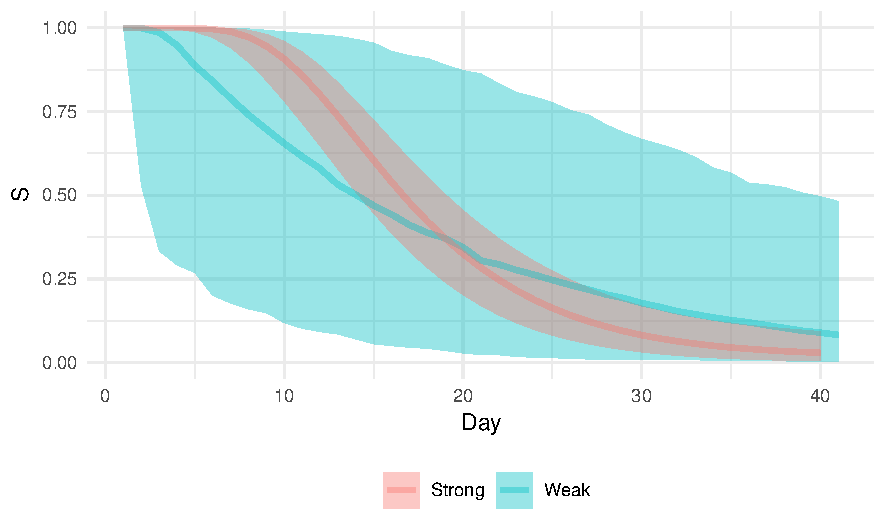
\includegraphics{figures/output/prior_predictive_survival}
  \caption{%
    Prior predictive values of $S_{\vec{\theta}}$ for the two priors.
  }
  \label{fig:priors}
\end{figure}

\subsection{Weakly informative prior}

The first prior for $S_{\vec{\theta}}$ is weakly informative, centered on prior estimates.
Specifically, we assume an independent prior distribution for each $\lambda_t$ of Beta(0.1, 1.9).
This distribution has mean 0.05, little information (standard deviation of 0.13), and a central 95\% probability mass of 0.00--0.47.
The mean is in line with previous estimates of the median duration~\citep{cevikShedding}.

\subsection{Strongly informative prior} \label{sec:ataccc-prior}

The second is a strongly informative prior; it incorporates prior information from reliable estimates of $\lambda_t$ for $t < 20$.
We take a previous Bayesian analysis~\citep{blakeThesis} of data from The Assessment of Transmission and Contagiousness of COVID-19 in Contacts (ATACCC) study~\citep{hakkiOnset}, which tested individuals who had been exposed to infection daily up to a maximum of 20 days.
This ATACCC-based analysis produces posterior estimates of $\lambda_t$ with a posterior distribution with positive correlation between $\lambda_t$ and $\lambda_{t'}$, especially for small $|t-t'|$.
Furthermore, the uncertainty in the prior estimates for $\lambda_t$ for $t\geq20$ are underestimated because they are based on extrapolation of the ATACCC data under strong model assumptions.

We first approximate the previous posterior estimate of the hazard as $\logit{\vec{h}} \dist \MNorm(\vec{\mu}_A, \matr{\Sigma}_A)$ where $\vec{h}$ is the hazard, and $\vec{\mu}_A$ and $\matr{\Sigma}_A$ are the mean and covariance matrix estimated using samples of $\logit{\vec{h}}$ from the previous study's posterior.
Using a multivariate normal, as opposed to multiple univariate distribution for each $h_t$, preserves the correlation between the hazards.
The approximation is very good (not shown).

Having approximated the estimate as a multivariate normal, we add additional uncertainty using a discrete Beta process.
The discrete Beta process prior~\citep{ibrahimBayesian,sunStatisticala} generalises the form of prior used in the weakly informative case by allowing the central estimate of the hazard to vary over time.
It is:
\begin{align}
  \logit \vec{h} &\dist \MNorm(\vec{\mu}_A, \matr{\Sigma}_A) \\
  \lambda_t &\dist \text{Beta}(\alpha_t, \beta_t) &t = 1, 2, \dots \\
  \alpha_t &= k_t h_t + \alpha_0 \\
  \beta_t &= k_t (1 - h_t) + \beta_0
\end{align}
where $k_t$, $\alpha_0$, and $\beta_0$ are hyperparameters.
An intuition for what this distribution represents derives from a conjugate model for $\lambda_t$ with a beta prior and a binomial likelihood.
If $\lambda_t$ is given the prior distribution $\text{Beta}(\alpha_0, \beta_0)$, and we then have $k_t$ observations with $k_t h_t$ successes, then the posterior distribution for $\lambda_t$ is $\text{Beta}(\alpha_t, \beta_t)$ (as defined above).
We use $\alpha_0 = 0.1$ and $\beta_0 = 1.9$ to match the weakly informative prior and the following form for $k_t$:
\begin{align}
k_t = \begin{cases}
  \expit(-0.4 \times (t - 20)) &\text{for $t \leq 39$} \\
  0 &t > 39.
\end{cases}
\end{align}
The form and choice of constants reflects the subjective belief that $h_t$ is a good estimate of $\lambda_t$ for small $t$ but increasingly unreliable; specifically, it is large at 0, when ATACCC is reliable, but becomes small for $t \geq 20$.

\section{Additional details of simulation study}

\subsection{Generation of data} \label{sec:simulation-data}

The algorithm for generating the data is as follows.

\begin{enumerate}
    \item Extract the test schedules for each individual who had at least one test during the period of interest.
    \item Draw an episode start time, $b_{j}$ for each individual uniformly at random between 2 July 2020 (100 days before the period where a detected episode would be included) and 6 December 2020 (the end of this period).
    \item Draw a duration of episode for their episode, $d_j$, based on a combination of previous estimates (described in \cref{sec:simulation-truth}). Then calculate the end of their infection episode, $e_{j} = b_{j} + d_i - 1$.
    \item Simulate the test results based on the test schedule, $b_{j}$, and $e_{j}$. A test on day $t$ between $b_{j}$ and $e_{j}$ (inclusive) is positive with probability $\psens$, where $\psens$ can vary with the time since infection, as defined below. All tests outside this interval are negative.
    \item Discard episodes where there are no positive tests (\ie undetected episodes) and then apply the inclusion criteria from \cref{sec:data}. Denote by $p$ the proportion of episodes that are retained.
    \item Of these remaining episodes, sample $\ndet = 4800$ to match the sample size of the true dataset. This is needed because in step 2 the entire cohort was infected, while in the real study only a (unknown) portion is infected.
    \item For this final set of episodes, calculate $(l_j^{(b)}, r_j^{(b)}, l_j^{(e)}, r_j^{(e)})$ by taking the day after the last negative prior to any positives, the first positive, the last positive, and the day before the negative following the last positive respectively.
\end{enumerate}

\section{Distribution of duration} \label{sec:simulation-truth}

The simulation requires a distribution of the duration of detectability.
We modify the ATACCC-based duration estimate from \citet[chapter 4]{blakeThesis} with an inflated tail to be consistent with the CIS.
The tail inflation uses a simple survival analysis and the CIS data.

This analysis assumes the initiating event is known, and equal to the episode’s detection time, $j_j^{(b)}$.
It assumes the final event is interval censored between the time of the final positive test and the subsequent negative test, or right censored if a negative test has not yet been observed.
A flexible, spline-based form is used for the baseline survival function~\citep{roystonSTPM,roystonFlexible} with covariates introduced via proportional odds.
By not accounting for either the undetected infections or the interval censoring of the initiating event, this analysis has competing biases which makes them hard to interpret~\citep{cisMethodsONS}.

To form the duration distribution used in the simulation, we combine the two estimates.
The pdf over the first 30 days is proportional to the ATACCC estimate, with the rest proportional to this CIS-based estimate.
Denote by $f_A(t)$ the ATACCC-based distribution function and $f_C(t)$ that from the CIS-based estimates just derived.
Then define:
$$
f_S'(t) = \begin{cases}
	f_A(t) &t \leq 30 \\
	f_C(t) &t > 30
\end{cases}
$$
Then the distribution used in the simulation is the normalised version of this: $f_S(t) = f'_S(t)/\sum_i f_S'(i)$.
% These curves and the combined curve are compared in \cref{perf-test:fig:duration-dist}.
Episode $j$'s duration of detectability is then a draw from this distribution.

\section{Additional figures}

\begin{figure}
  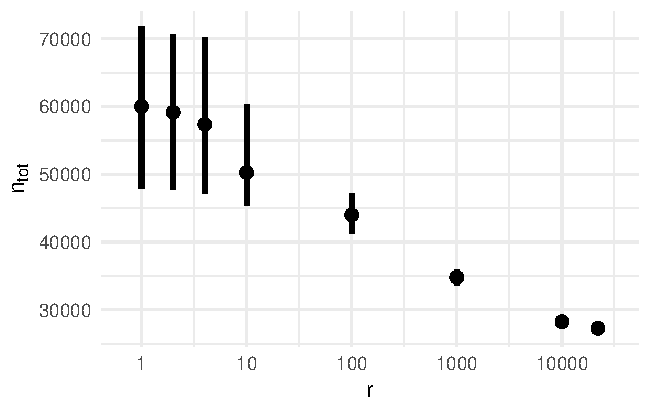
\includegraphics{figures/output/CIS_ntot}
  \caption[Sensitivity of $\ntot$'s posterior to its prior.]{How the posterior estimate of $\ntot$ changes with the value of $r$ in the prior on $\ntot$.}
  \label{imperf-test:fig:ntot}
\end{figure}

\bibliographystyle{agsm}

\bibliography{references}

\end{document}